\setcolumnwidth{44mm, 130mm}
\setlength{\columnsep}{8mm}

\begin{paracol}{2}
\switchcolumn[1]
\noindent Thay $h = 3\text{ m}$ và $dV/dt = 2\text{ m}^3/\text{phút}$, ta có
\[
\frac{dh}{dt} = \frac{4}{\pi(3)^2} \cdot 2 = \frac{8}{9\pi}
\]
Mực nước đang dâng lên với tốc độ $8/(9\pi) \approx 0{,}28\text{ m/phút}$.\stewartqed

\vspace{1em}
\noindent\textbf{\color{stewartblue}VÍ DỤ 4}\quad Xe A đang chạy về phía tây với tốc độ $50\text{ mi/h}$ và xe B đang chạy về phía bắc với tốc độ $60\text{ mi/h}$. Cả hai xe đều đang hướng về phía giao lộ của hai con đường. Hỏi hai xe đang tiến lại gần nhau với tốc độ bao nhiêu khi xe A cách giao lộ $0{,}3\text{ mi}$ và xe B cách giao lộ $0{,}4\text{ mi}$?

\switchcolumn[0]*
\noindent
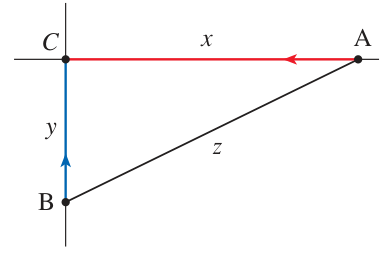
\includegraphics[width=\linewidth]{images/p0285_fig1.png}\par
\vspace{4pt}
\noindent{\footnotesize\textsf{\textbf{\color{stewartblue}HÌNH 4}}}

\switchcolumn[1]
\noindent\textbf{\color{stewartblue}LỜI GIẢI}\quad Ta vẽ Hình 4, trong đó $C$ là giao lộ của hai con đường. Tại một thời điểm $t$ đã cho, gọi $x$ là khoảng cách từ xe A đến $C$, $y$ là khoảng cách từ xe B đến $C$, và $z$ là khoảng cách giữa hai xe, với $x$, $y$ và $z$ được tính bằng dặm ($\text{mi}$).

Theo giả thiết, ta có $dx/dt = -50\text{ mi/h}$ và $dy/dt = -60\text{ mi/h}$. (Các đạo hàm mang dấu âm vì $x$ và $y$ đang giảm dần.) Ta cần tìm $dz/dt$. Phương trình liên hệ giữa $x$, $y$ và $z$ được cho bởi định lý Pythagore:
\[
z^2 = x^2 + y^2
\]
Lấy đạo hàm hai vế theo $t$, ta có
\[
2z \frac{dz}{dt} = 2x \frac{dx}{dt} + 2y \frac{dy}{dt}
\]
\[
\frac{dz}{dt} = \frac{1}{z} \left( x \frac{dx}{dt} + y \frac{dy}{dt} \right)
\]
Khi $x = 0{,}3\text{ mi}$ và $y = 0{,}4\text{ mi}$, định lý Pythagore cho ta $z = 0{,}5\text{ mi}$, do đó
\[
\frac{dz}{dt} = \frac{1}{0{,}5} [0{,}3(-50) + 0{,}4(-60)] = -78\text{ mi/h}
\]
Hai xe đang tiến lại gần nhau với tốc độ $78\text{ mi/h}$.\stewartqed

\vspace{1em}
\noindent\textbf{\color{stewartblue}VÍ DỤ 5}\quad Một người đàn ông đi bộ dọc theo một đường thẳng với tốc độ $4\text{ ft/s}$. Một ngọn đèn rọi đặt trên mặt đất cách con đường $20\text{ ft}$ và luôn chiếu thẳng vào người đàn ông. Đèn rọi đang quay với tốc độ bằng bao nhiêu khi người đàn ông cách điểm trên đường gần đèn nhất $15\text{ ft}$?

\vspace{0.5em}
\noindent\textbf{\color{stewartblue}LỜI GIẢI}\quad Ta vẽ Hình 5 và gọi $x$ là khoảng cách từ người đàn ông đến điểm trên đường gần đèn rọi nhất. Gọi $\theta$ là góc giữa chùm sáng và đường vuông góc với đường đi.

Theo giả thiết, ta có $dx/dt = 4\text{ ft/s}$ và cần tìm $d\theta/dt$ khi $x = 15$. Phương trình liên hệ giữa $x$ và $\theta$ có thể viết từ Hình 5:

\switchcolumn[0]*
\noindent
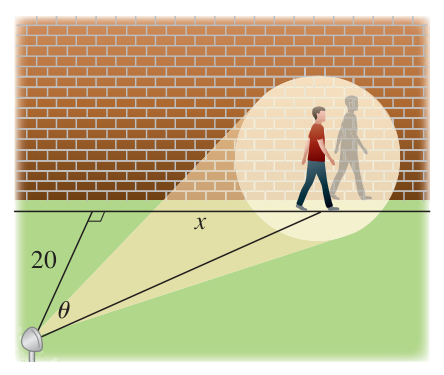
\includegraphics[width=\linewidth]{images/p0285_fig2.png}\par
\vspace{4pt}
\noindent{\footnotesize\textsf{\textbf{\color{stewartblue}HÌNH 5}}}

\switchcolumn[1]
\[
\frac{x}{20} = \tan \theta \qquad x = 20 \tan \theta
\]
Lấy đạo hàm hai vế theo $t$, ta được
\[
\frac{dx}{dt} = 20 \sec^2 \theta \frac{d\theta}{dt}
\]
do đó
\[
\begin{aligned}
\frac{d\theta}{dt} &= \frac{1}{20} \cos^2 \theta \frac{dx}{dt} \\[6pt]
&= \frac{1}{20} \cos^2 \theta \,(4) = \frac{1}{5} \cos^2 \theta
\end{aligned}
\]
\end{paracol}
